% Options for packages loaded elsewhere
% Options for packages loaded elsewhere
\PassOptionsToPackage{unicode}{hyperref}
\PassOptionsToPackage{hyphens}{url}
\PassOptionsToPackage{dvipsnames,svgnames,x11names}{xcolor}
%
\documentclass[
  letterpaper,
  DIV=11,
  numbers=noendperiod]{scrreprt}
\usepackage{xcolor}
\usepackage{amsmath,amssymb}
\setcounter{secnumdepth}{5}
\usepackage{iftex}
\ifPDFTeX
  \usepackage[T1]{fontenc}
  \usepackage[utf8]{inputenc}
  \usepackage{textcomp} % provide euro and other symbols
\else % if luatex or xetex
  \usepackage{unicode-math} % this also loads fontspec
  \defaultfontfeatures{Scale=MatchLowercase}
  \defaultfontfeatures[\rmfamily]{Ligatures=TeX,Scale=1}
\fi
\usepackage{lmodern}
\ifPDFTeX\else
  % xetex/luatex font selection
\fi
% Use upquote if available, for straight quotes in verbatim environments
\IfFileExists{upquote.sty}{\usepackage{upquote}}{}
\IfFileExists{microtype.sty}{% use microtype if available
  \usepackage[]{microtype}
  \UseMicrotypeSet[protrusion]{basicmath} % disable protrusion for tt fonts
}{}
\makeatletter
\@ifundefined{KOMAClassName}{% if non-KOMA class
  \IfFileExists{parskip.sty}{%
    \usepackage{parskip}
  }{% else
    \setlength{\parindent}{0pt}
    \setlength{\parskip}{6pt plus 2pt minus 1pt}}
}{% if KOMA class
  \KOMAoptions{parskip=half}}
\makeatother
% Make \paragraph and \subparagraph free-standing
\makeatletter
\ifx\paragraph\undefined\else
  \let\oldparagraph\paragraph
  \renewcommand{\paragraph}{
    \@ifstar
      \xxxParagraphStar
      \xxxParagraphNoStar
  }
  \newcommand{\xxxParagraphStar}[1]{\oldparagraph*{#1}\mbox{}}
  \newcommand{\xxxParagraphNoStar}[1]{\oldparagraph{#1}\mbox{}}
\fi
\ifx\subparagraph\undefined\else
  \let\oldsubparagraph\subparagraph
  \renewcommand{\subparagraph}{
    \@ifstar
      \xxxSubParagraphStar
      \xxxSubParagraphNoStar
  }
  \newcommand{\xxxSubParagraphStar}[1]{\oldsubparagraph*{#1}\mbox{}}
  \newcommand{\xxxSubParagraphNoStar}[1]{\oldsubparagraph{#1}\mbox{}}
\fi
\makeatother

\usepackage{color}
\usepackage{fancyvrb}
\newcommand{\VerbBar}{|}
\newcommand{\VERB}{\Verb[commandchars=\\\{\}]}
\DefineVerbatimEnvironment{Highlighting}{Verbatim}{commandchars=\\\{\}}
% Add ',fontsize=\small' for more characters per line
\usepackage{framed}
\definecolor{shadecolor}{RGB}{241,243,245}
\newenvironment{Shaded}{\begin{snugshade}}{\end{snugshade}}
\newcommand{\AlertTok}[1]{\textcolor[rgb]{0.68,0.00,0.00}{#1}}
\newcommand{\AnnotationTok}[1]{\textcolor[rgb]{0.37,0.37,0.37}{#1}}
\newcommand{\AttributeTok}[1]{\textcolor[rgb]{0.40,0.45,0.13}{#1}}
\newcommand{\BaseNTok}[1]{\textcolor[rgb]{0.68,0.00,0.00}{#1}}
\newcommand{\BuiltInTok}[1]{\textcolor[rgb]{0.00,0.23,0.31}{#1}}
\newcommand{\CharTok}[1]{\textcolor[rgb]{0.13,0.47,0.30}{#1}}
\newcommand{\CommentTok}[1]{\textcolor[rgb]{0.37,0.37,0.37}{#1}}
\newcommand{\CommentVarTok}[1]{\textcolor[rgb]{0.37,0.37,0.37}{\textit{#1}}}
\newcommand{\ConstantTok}[1]{\textcolor[rgb]{0.56,0.35,0.01}{#1}}
\newcommand{\ControlFlowTok}[1]{\textcolor[rgb]{0.00,0.23,0.31}{\textbf{#1}}}
\newcommand{\DataTypeTok}[1]{\textcolor[rgb]{0.68,0.00,0.00}{#1}}
\newcommand{\DecValTok}[1]{\textcolor[rgb]{0.68,0.00,0.00}{#1}}
\newcommand{\DocumentationTok}[1]{\textcolor[rgb]{0.37,0.37,0.37}{\textit{#1}}}
\newcommand{\ErrorTok}[1]{\textcolor[rgb]{0.68,0.00,0.00}{#1}}
\newcommand{\ExtensionTok}[1]{\textcolor[rgb]{0.00,0.23,0.31}{#1}}
\newcommand{\FloatTok}[1]{\textcolor[rgb]{0.68,0.00,0.00}{#1}}
\newcommand{\FunctionTok}[1]{\textcolor[rgb]{0.28,0.35,0.67}{#1}}
\newcommand{\ImportTok}[1]{\textcolor[rgb]{0.00,0.46,0.62}{#1}}
\newcommand{\InformationTok}[1]{\textcolor[rgb]{0.37,0.37,0.37}{#1}}
\newcommand{\KeywordTok}[1]{\textcolor[rgb]{0.00,0.23,0.31}{\textbf{#1}}}
\newcommand{\NormalTok}[1]{\textcolor[rgb]{0.00,0.23,0.31}{#1}}
\newcommand{\OperatorTok}[1]{\textcolor[rgb]{0.37,0.37,0.37}{#1}}
\newcommand{\OtherTok}[1]{\textcolor[rgb]{0.00,0.23,0.31}{#1}}
\newcommand{\PreprocessorTok}[1]{\textcolor[rgb]{0.68,0.00,0.00}{#1}}
\newcommand{\RegionMarkerTok}[1]{\textcolor[rgb]{0.00,0.23,0.31}{#1}}
\newcommand{\SpecialCharTok}[1]{\textcolor[rgb]{0.37,0.37,0.37}{#1}}
\newcommand{\SpecialStringTok}[1]{\textcolor[rgb]{0.13,0.47,0.30}{#1}}
\newcommand{\StringTok}[1]{\textcolor[rgb]{0.13,0.47,0.30}{#1}}
\newcommand{\VariableTok}[1]{\textcolor[rgb]{0.07,0.07,0.07}{#1}}
\newcommand{\VerbatimStringTok}[1]{\textcolor[rgb]{0.13,0.47,0.30}{#1}}
\newcommand{\WarningTok}[1]{\textcolor[rgb]{0.37,0.37,0.37}{\textit{#1}}}

\usepackage{longtable,booktabs,array}
\newcounter{none} % for unnumbered tables
\usepackage{calc} % for calculating minipage widths
% Correct order of tables after \paragraph or \subparagraph
\usepackage{etoolbox}
\makeatletter
\patchcmd\longtable{\par}{\if@noskipsec\mbox{}\fi\par}{}{}
\makeatother
% Allow footnotes in longtable head/foot
\IfFileExists{footnotehyper.sty}{\usepackage{footnotehyper}}{\usepackage{footnote}}
\makesavenoteenv{longtable}
\usepackage{graphicx}
\makeatletter
\newsavebox\pandoc@box
\newcommand*\pandocbounded[1]{% scales image to fit in text height/width
  \sbox\pandoc@box{#1}%
  \Gscale@div\@tempa{\textheight}{\dimexpr\ht\pandoc@box+\dp\pandoc@box\relax}%
  \Gscale@div\@tempb{\linewidth}{\wd\pandoc@box}%
  \ifdim\@tempb\p@<\@tempa\p@\let\@tempa\@tempb\fi% select the smaller of both
  \ifdim\@tempa\p@<\p@\scalebox{\@tempa}{\usebox\pandoc@box}%
  \else\usebox{\pandoc@box}%
  \fi%
}
% Set default figure placement to htbp
\def\fps@figure{htbp}
\makeatother





\setlength{\emergencystretch}{3em} % prevent overfull lines

\providecommand{\tightlist}{%
  \setlength{\itemsep}{0pt}\setlength{\parskip}{0pt}}



 


\KOMAoption{captions}{tableheading}
\makeatletter
\@ifpackageloaded{tcolorbox}{}{\usepackage[skins,breakable]{tcolorbox}}
\@ifpackageloaded{fontawesome5}{}{\usepackage{fontawesome5}}
\definecolor{quarto-callout-color}{HTML}{909090}
\definecolor{quarto-callout-note-color}{HTML}{0758E5}
\definecolor{quarto-callout-important-color}{HTML}{CC1914}
\definecolor{quarto-callout-warning-color}{HTML}{EB9113}
\definecolor{quarto-callout-tip-color}{HTML}{00A047}
\definecolor{quarto-callout-caution-color}{HTML}{FC5300}
\definecolor{quarto-callout-color-frame}{HTML}{acacac}
\definecolor{quarto-callout-note-color-frame}{HTML}{4582ec}
\definecolor{quarto-callout-important-color-frame}{HTML}{d9534f}
\definecolor{quarto-callout-warning-color-frame}{HTML}{f0ad4e}
\definecolor{quarto-callout-tip-color-frame}{HTML}{02b875}
\definecolor{quarto-callout-caution-color-frame}{HTML}{fd7e14}
\makeatother
\makeatletter
\@ifpackageloaded{bookmark}{}{\usepackage{bookmark}}
\makeatother
\makeatletter
\@ifpackageloaded{caption}{}{\usepackage{caption}}
\AtBeginDocument{%
\ifdefined\contentsname
  \renewcommand*\contentsname{Table of contents}
\else
  \newcommand\contentsname{Table of contents}
\fi
\ifdefined\listfigurename
  \renewcommand*\listfigurename{List of Figures}
\else
  \newcommand\listfigurename{List of Figures}
\fi
\ifdefined\listtablename
  \renewcommand*\listtablename{List of Tables}
\else
  \newcommand\listtablename{List of Tables}
\fi
\ifdefined\figurename
  \renewcommand*\figurename{Figure}
\else
  \newcommand\figurename{Figure}
\fi
\ifdefined\tablename
  \renewcommand*\tablename{Table}
\else
  \newcommand\tablename{Table}
\fi
}
\@ifpackageloaded{float}{}{\usepackage{float}}
\floatstyle{ruled}
\@ifundefined{c@chapter}{\newfloat{codelisting}{h}{lop}}{\newfloat{codelisting}{h}{lop}[chapter]}
\floatname{codelisting}{Listing}
\newcommand*\listoflistings{\listof{codelisting}{List of Listings}}
\makeatother
\makeatletter
\makeatother
\makeatletter
\@ifpackageloaded{caption}{}{\usepackage{caption}}
\@ifpackageloaded{subcaption}{}{\usepackage{subcaption}}
\makeatother
\usepackage{bookmark}
\IfFileExists{xurl.sty}{\usepackage{xurl}}{} % add URL line breaks if available
\urlstyle{same}
\hypersetup{
  pdftitle={Aero 5553 - Advanced Control Theory},
  pdfauthor={Eric A. Mehiel, Ph.D.},
  colorlinks=true,
  linkcolor={blue},
  filecolor={Maroon},
  citecolor={Blue},
  urlcolor={Blue},
  pdfcreator={LaTeX via pandoc}}


\title{Aero 5553 - Advanced Control Theory}
\usepackage{etoolbox}
\makeatletter
\providecommand{\subtitle}[1]{% add subtitle to \maketitle
  \apptocmd{\@title}{\par {\large #1 \par}}{}{}
}
\makeatother
\subtitle{Course Notes}
\author{Eric A. Mehiel, Ph.D.}
\date{}
\begin{document}
\maketitle

\renewcommand*\contentsname{Table of contents}
{
\setcounter{tocdepth}{2}
\tableofcontents
}

\bookmarksetup{startatroot}

\chapter{Preface}\label{preface}

These notes accompany a graduate course in Advanced Control Systems at
Cal Poly, San Luis Obispo. The course is taught by Dr.~E. Mehiel and is
based on several books. Primarily, the course is based on the book,

\begin{itemize}
\tightlist
\item
  ``Feedback Systems: An Introduction for Scientists and Engineers'' by
  Karl J. Åström and Richard M. Murray, Princeton University Press,
  2008,
\item
  ``Linear System Theory: Second Edition'' by J. Hespanha, Princeton
  University Press, 2018,
\item
  ``Robust and Adaptive Control: With Aerospace Applications'' by E.
  Lavretsky and K. Wise, Springer, 2013.
\end{itemize}

The course is designed to provide students with a solid foundation in
modern control theory and its applications.

Each chapter contains:

\begin{itemize}
\tightlist
\item
  Learning objectives
\item
  Theory
\item
  Worked examples
\item
  Summary
\item
  Exercises
\end{itemize}

\bookmarksetup{startatroot}

\chapter{Dynamic System Control}\label{dynamic-system-control}

\section{Slide 2 - Motivation and Learning
Outcomes}\label{slide-2---motivation-and-learning-outcomes}

\subsection{Motivation}\label{motivation}

\begin{itemize}
\tightlist
\item
  Control is just ``making things work.''
\item
  From a physics perspective the difference between an uncontrolled and
  controlled dynamic system is irrelevant
\item
  From an engineering perspective, the difference between the two is
  central to design and performance
\item
  But the mathematical techniques are the same, so, it's theory\ldots{}

  \begin{itemize}
  \tightlist
  \item
    Control theory is the mathematical formalism we use to analyze and
    design (engineer) dynamic systems (things that move).
  \end{itemize}
\item
  https://en.wikipedia.org/wiki/Control\_theory
\end{itemize}

\subsection{Learning Outcomes}\label{learning-outcomes}

\begin{itemize}
\tightlist
\item
  Look inside the `mind' of a controls engineer
\item
  Discuss important concepts, like feedback, robustness, and Automation
\item
  Develop a conceptual understanding of PID control
\end{itemize}

\section{Slide 3 - The `mind' of a controls
engineer}\label{slide-3---the-mind-of-a-controls-engineer}

\section{Slide 4 - What is feedback?}\label{slide-4---what-is-feedback}

When we develop models of dynamic systems with differential equations,
other math and physics, we take a reductive approach. When two or more
dynamical systems are connected in a way where both systems depend on
output from the other system for input, the dynamical systems are in
\emph{feedback}.

Another way of thinking about feedback is that the connected systems
cannot be solved independently from each other. The systems are
\emph{coupled} and must be solved together.

\section{Slide 5 - The Centrifugal
Governor}\label{slide-5---the-centrifugal-governor}

An early example of feedback is the centrifugal governor, which was used
to control the speed of steam engines. The governor uses feedback to
adjust the fuel supply to the engine based on its speed, maintaining a
desired speed despite changes in load.

\section{Slide 6 - Steam Engine as a Block
Diagram}\label{slide-6---steam-engine-as-a-block-diagram}

Block diagrams are a way to represent the relationships between
different components of a system. The steam engine can be represented as
a block diagram, with the governor and engine as separate blocks that
interact through feedback.

This is a reductive approach to modeling the system which it allows us
to analyze and design the system more easily.

Early object oriented programming was based on this idea of modeling
systems as blocks that interact with each other. Modelica is a modern
programming language that uses this approach to model complex systems.

\section{Slide 7 - Cruise Control}\label{slide-7---cruise-control}

Cruise control is a common example of feedback control in modern
vehicles. The system uses feedback from the vehicle's speed to adjust
the throttle and maintain a desired speed, even when going up or down
hills.

Cruise control systems started as mechanical systems, but have since
evolved into computer-controlled systems that use sensors and algorithms
to optimize performance and fuel efficiency.

\section{Slide 8 - Biological and Ecological
Systems}\label{slide-8---biological-and-ecological-systems}

Control theory is not limited to mechanical or electrical systems.
Biological and ecological systems also exhibit feedback control, such as
the complex chemical systems of cells and how birds fly in formation.

With the advent of mechanical systems and now computer systems, we can
design or program a feedback loop.

These days control is a mix of design and computer control with embedded
or other computer systems.

\section{Slide 9 - Feedback
Properties}\label{slide-9---feedback-properties}

\begin{itemize}
\tightlist
\item
  Robustness -- As mass increases, the car still gets to the desired
  speed in roughly the same amount of time but with different
  ``performance''.

  \begin{itemize}
  \tightlist
  \item
    Question how much fuel is used? So the cruise control is robust, but
    there is no consideration of energy.
  \end{itemize}
\item
  Design of Dynamics - Use feedback control to change the closed-loop
  dynamics of the system. Design a vehicle for some set of requirements,
  and design a controller to meet performance metrics. Example, the
  Wright Flyer.
\item
  Automation - Combining control theory and dynamics with logic,
  heuristics, or AI to achieve more complicated control objectives or
  enhanced performance or robustness.
\end{itemize}

\section{Slide 10 - Some Notes}\label{slide-10---some-notes}

\section{Slide 11 - PID: An Intuitive Approach for Linear
Systems}\label{slide-11---pid-an-intuitive-approach-for-linear-systems}

\begin{itemize}
\tightlist
\item
  Proportional - Control for right now
\item
  Derivative - Control for the expecte future
\item
  Integral - Control for the past
\item
  PID - a blend of all three time lines - this works because of Newton's
  Laws. How you ended up in your current state is a function of where
  you were (I), the decision you make right now (P), and where you want
  to go (D).
\end{itemize}

\section{Slide 12 - Buckaroo Banzi}\label{slide-12---buckaroo-banzi}

``No matter how much you push the envelope, it'll still be stationery.''
- Buckaroo Banzai

``No matter where you go, there you are.'' - Buckaroo Banzai

\section{Slide 13 - Control Theory Mind
Map}\label{slide-13---control-theory-mind-map}

Where are we going in this class?

\bookmarksetup{startatroot}

\chapter{Classical Control
Highlights}\label{classical-control-highlights}

\section{Slide 2 - Motivation and Learning
Outcomes}\label{slide-2---motivation-and-learning-outcomes-1}

\subsection{Motivation}\label{motivation-1}

\begin{itemize}
\tightlist
\item
  Proportional, Integral, Derivative Control
\item
  For ``single-input, single-output'' systems, PID is often sufficient
\item
  PID has been around a long time and is well understood
\item
  PID is relatively easy to tune with decent performance for linear
  systems
\item
  Classical Control is done in the ``s-domain'' (or frequency or Laplace
  Domain)
\item
  However, PID is not the best choice for non-linear, time-varying, or
  multi-input, multi-output, or complex systems
\end{itemize}

\subsection{Learning Outcomes}\label{learning-outcomes-1}

\begin{itemize}
\tightlist
\item
  Review the Laplace domain and its use in control systems
\item
  Relate solutions of linear ODEs to concepts like, stabilty and
  peroformance
\item
  Look into the concepts of propotional, integral, and derivative
  control
\end{itemize}

\section{Slide 3 - Functions of a Complex
Variable}\label{slide-3---functions-of-a-complex-variable}

Let \(s=a+jb\) be a complex number with \(j=\sqrt{-1}\). Notice we
typically use \(j\) in controls since the Electrical Engineers took
\(i\) for current.

We define the \emph{rational polynomial} \(G(s)\) as:

\[G(s) = \frac{a_0s^m+ a_1s^{m-1} + \cdots + a_m}{s^n+b_1s^{n-1}+ \cdots + b_n}\]
\[= \frac{N(s)}{D(s)}, \ for \ a_i, \ b_i \in \mathbb{R}\]

When \(m<n\), we say that \(G(s)\) is \emph{strictly proper}. When
\(m=n\), we say that \(G(s)\) is \emph{proper}. When \(m>n\), we say
that \(G(s)\) is \emph{improper}.

If we factor \(G(s)\) into its roots, we can write:

\$\(G(s) = K\frac{(s-z_1)(s-z_2)\cdots(s-z_m)}{(s-p_1)(s-p_2)\cdots(s-p_n)}\)

where \(z_i\) are the \emph{zeros} of \(G(s)\) and \(p_i\) are the
\emph{poles} of \(G(s)\).

Notice that the poles and zeros are complex numbers, and that the poles
are the roots of the denominator polynomial \(D(s)\) and the zeros are
the roots of the numerator polynomial \(N(s)\).

In set from \({z_i}\) = \{s \textbar{} N(s) = 0\} and \({p_i}\) = \{s
\textbar{} D(s) = 0\}. The \emph{order} of \(G(s)\) is the number of
poles, \(n\).

\section{Slide 4 - Poles and Zeros
Examples}\label{slide-4---poles-and-zeros-examples}

\[G(s) = \frac{(s+2)(s+10)}{s(s+5)(s+15)^2}\]

Therefore,

\[z = \left\{ -2, -10 \right\}\]

\[p = \{0, -5, -15, -15\}\]

Another more complex example is:

\[ G(s) = \frac{(s + 2)(s^2 + s + 5)}{s (s + 5)(s^2 + 5s + 15)}\]

\begin{Shaded}
\begin{Highlighting}[]
\ImportTok{import}\NormalTok{ numpy }\ImportTok{as}\NormalTok{ np}
\ImportTok{import}\NormalTok{ matplotlib.pyplot }\ImportTok{as}\NormalTok{ plt}
\ImportTok{import}\NormalTok{ control }\ImportTok{as}\NormalTok{ ct}

\CommentTok{\# Define the transfer function: G(s) = (s+2)(s\^{}2+s+5) / (s(s+5)(s\^{}2+5s+15))}
\NormalTok{num }\OperatorTok{=}\NormalTok{ np.polymul([}\DecValTok{1}\NormalTok{, }\DecValTok{2}\NormalTok{], [}\DecValTok{1}\NormalTok{, }\DecValTok{1}\NormalTok{, }\DecValTok{5}\NormalTok{])}
\NormalTok{den }\OperatorTok{=}\NormalTok{ np.polymul([}\DecValTok{1}\NormalTok{, }\DecValTok{0}\NormalTok{], np.polymul([}\DecValTok{1}\NormalTok{, }\DecValTok{5}\NormalTok{], np.polymul([}\DecValTok{1}\NormalTok{, }\DecValTok{5}\NormalTok{, }\DecValTok{15}\NormalTok{], [}\DecValTok{1}\NormalTok{, }\DecValTok{5}\NormalTok{, }\DecValTok{15}\NormalTok{])))}
\NormalTok{G }\OperatorTok{=}\NormalTok{ ct.TransferFunction(num, den)}

\CommentTok{\# Plot the poles and zeros}
\NormalTok{plt.figure()}
\NormalTok{ct.pole\_zero\_plot(G, title}\OperatorTok{=}\StringTok{\textquotesingle{}Poles and Zeros of G(s)\textquotesingle{}}\NormalTok{, grid}\OperatorTok{=}\VariableTok{True}\NormalTok{)}
\NormalTok{plt.show()}
\end{Highlighting}
\end{Shaded}

\pandocbounded{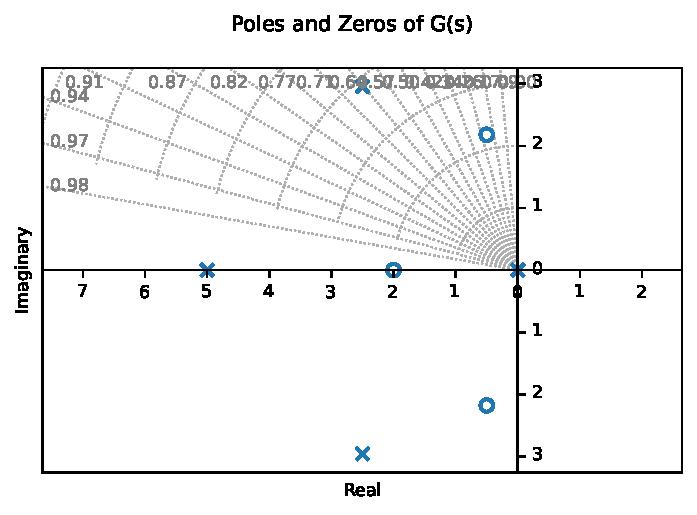
\includegraphics[keepaspectratio]{chapters/01_1-classical-control-highlights_files/figure-pdf/cell-2-output-1.pdf}}

\section{Slide 5 - The Laplace
Transform}\label{slide-5---the-laplace-transform}

The Laplace transform converts a time-domain signal into the complex
frequency domain. For a causal function \(f(t)\) (defined for \(t\ge0\))
the unilateral Laplace transform is

\[F(s)=\mathcal{L}\{f(t)\}=\int_{0}^{\infty} e^{-st}f(t)\,dt\],

where \(s=\sigma+j\omega\) is a complex variable and the integral
converges in the region of convergence (ROC).

Drawing of mapping from time domain to s-domain and back.

\section{Slide 6 - Properties of the Laplace
Transform}\label{slide-6---properties-of-the-laplace-transform}

Key properties:

\begin{itemize}
\tightlist
\item
  Linearity: \(\mathcal{L}\{a f(t)+b g(t)\}=aF(s)+bG(s)\).
\item
  Time shift: \(\mathcal{L}\{f(t-a)u(t-a)\}=e^{-as}F(s)\).
\item
  Frequency shift: \(\mathcal{L}\{e^{at}f(t)\}=F(s-a)\).
\item
  Differentiation (time): \(\mathcal{L}\{f'(t)\}=sF(s)-f(0^+)\).
\item
  Differentiation (time, higher order):
  \(\mathcal{L}\{f^{(n)}(t)\}=s^nF(s)-s^{n-1}f(0^+)-\cdots-f^{(n-1)}(0^+)\).
\item
  Integration (time):
  \(\mathcal{L}\{\int_0^t f(\tau)\,d\tau\}=\frac{1}{s}F(s)\).
\item
  Integration (time, higher order):
  \(\mathcal{L}\{\int_0^t \int_0^{\tau_1} \cdots \int_0^{\tau_{n-1}} f(\tau_n)\,d\tau_n \cdots d\tau_2 d\tau_1\}=\frac{1}{s^n}F(s)\).
\end{itemize}

Common transforms (causal signals):

\begin{itemize}
\item
  \(\mathcal{L}\{1\}=\dfrac{1}{s}\)
\item
  \(\mathcal{L}\{t\}=\dfrac{1}{s^{2}}\)
\item
  \(\mathcal{L}\{e^{at}\}=\dfrac{1}{s-a}\)
\item
  \(\mathcal{L}\{\sin(\omega t)\}=\dfrac{\omega}{s^{2}+\omega^{2}}\)
\item
  \(\mathcal{L}\{\cos(\omega t)\}=\dfrac{s}{s^{2}+\omega^{2}}\)
\end{itemize}

\section{Slide 7 - Useful Theorems}\label{slide-7---useful-theorems}

Useful theorems:

\begin{itemize}
\tightlist
\item
  Initial value theorem: \(f(0^+)=\lim_{s\to\infty} sF(s)\).
\item
  Final value theorem: \(\lim_{t\to\infty} f(t)=\lim_{s\to0} sF(s)\),
  when the limits exist (i.e., poles of \(sF(s)\) are in the left
  half-plane).
\end{itemize}

Quick example: \(f(t)=e^{2t}u(t)\) has transform \(F(s)=1/(s-2)\) for
\(\mathrm{Re}(s)>2\).

The Laplace transform is fundamental in linear systems analysis because
it turns linear differential equations into algebraic equations in
\(s\), simplifying solution and control-design tasks.

\section{Slide 8 - Why Laplace?}\label{slide-8---why-laplace}

One way to think about the Laplace transform is that it is a
generalization of the Fourier transform. The Fourier transform is a
special case of the Laplace transform where \(s=j\omega\) and
\(\sigma=0\). The Laplace transform allows us to analyze systems with
exponential growth or decay, which is common in control systems.

The Laplace Transform is helpful because it transforms differential
equations into algebraic equations, making it easier to analyze and
design control systems.

If we can solve the algebraic equations in the Laplace domain, we can
then use the inverse Laplace transform to find the solution in the time
domain.

\subsection{Example - Mass-Spring-Damper System
(MSD)}\label{example---mass-spring-damper-system-msd}

Figure of MSD

The equation of motion for a mass-spring-damper system is given by:

\[ m\ddot{x}(t) + c\dot{x}(t) + kx(t) = F(t)\]

Let \(\omega_n^2 = {k/m}\) where \(\omega_n\) is the natural frequency,
and \(\frac{c}{m} = 2\zeta\omega_n\), so
\(\zeta = \frac{c}{2\sqrt{mk}}\) is the damping ratio, and \(F=k u(t)\)
is the force required to displace the mass some distance, \(u(t)\)
acoring to Hook's law. Finally, divide both sides by \(m\) to get:

\[ \ddot{x}(t) + 2\zeta\omega_n \dot{x}(t) + \omega_n^2 x(t) = \omega_n^2 u(t) \]

Now, define the state vector as
\(\underline{x}(t) = \begin{bmatrix} x(t) \\ \dot{x}(t) \end{bmatrix}\),
and we can write the system in state-space form as:

\[ \dot{\underline{x}}(t) = \begin{bmatrix} 0 & 1 \\ -\omega_n^2 & -2\zeta\omega_n \end{bmatrix} \underline{x}(t) + \begin{bmatrix} 0 \\ \omega_n^2 \end{bmatrix} \underline{u}(t) \]

In more compact form, we can write this as:

\[ \dot{\underline{x}}(t) = A\underline{x}(t) + B \underline{u}(t) \]

This is known as the state-space representation or state equation of the
system, where \(A\) is the system matrix and \(B\) is the input matrix.

where
\(A = \begin{bmatrix} 0 & 1 \\ -\omega_n^2 & -2\zeta\omega_n \end{bmatrix}\)
and \(B = \begin{bmatrix} 0 \\ \omega_n^2 \end{bmatrix}\).

Assuming we measure the position of the mass, we can define the output
as \[y(t) = C\underline{x}(t)\]

where \(C = \begin{bmatrix} 1 & 0 \end{bmatrix}\). This is know as the
\emph{output} or measurement equation of the system.

In control theory, we can generally let the output be a function of the
input, i.e.,
\(\underline{y}(t) = C\underline{x}(t) + D\underline{u}(t)\), where
\(D\) is a \emph{feed through} term. In this case, we have no \emph{feed
through}, so \(D=0\).

Now, we can take the Laplace transform of the state-space equations to
get:

\[\mathcal{L}\{\dot{\underline{x}}(t)\} = \mathcal{L}\{A\underline{x}(t) + B\underline{u}(t)\}\]

\[ s\underline{X}(s) - \underline{x}(0) = A\underline{X}(s) + B\underline{U}(s) \]

where \(\underline{X}(s)\) is the Laplace transform of the state vector
\(\underline{x}(t)\), and \(\underline{U}(s)\) is the Laplace transform
of the input vector \(\underline{u}(t)\).

Assuming \(\underline{x}(0) = 0\), we can solve for
\(\underline{X}(s)\):

\[ \underline{X}(s) = (sI - A)^{-1}B\underline{U}(s) \]

Finally, we can find the output in the Laplace domain:
\[ \underline{Y}(s) = C\underline{X}(s) = C(sI - A)^{-1}B\underline{U}(s) \]

We define the \emph{transfer function} of the system \(G(s)\) as the
ratio of the output to the input in the Laplace domain:

\[ G(s) = \frac{\underline{Y}(s)}{\underline{U}(s)} = C(sI - A)^{-1}B \]

From before we notice,

\[ G(s) = \frac{N(s)}{D(s)}\]

Therefore,

\[ Y(s) = G(s)U(s) = C(sI - A)^{-1}BU(s) = \frac{N(s)}{D(s)}\]

\section{Slide 9 - Another look at the Transfer
Function}\label{slide-9---another-look-at-the-transfer-function}

The transfer function is,

\[ G(s) = \frac{N(s)}{D(s)}\]

Recall that for any matrix \(P\), the inverse of \(P\) is given by,

\[ P^{-1} = \frac{adj(P)}{det(P)}\]

where \(adj(P)\) is the adjugate of \(P\) and \(det(P)\) is the
determinant of \(P\).

The adjugate of a matrix is the conjugate transpose of the cofactor
matrix.

This is the least efficient way to compute the inverse of a matrix, but
it is useful for theoretical analysis.

Notice the adugate is a matrix of polynomials in \(s\), and is
\(n \times n\) where \(n\) is the order of the system. The determinant
is a polynomial in \(s\) of order \(n\). Therefore, we can write,

\[ (sI - A)^{-1} = \frac{adj(sI - A)}{det(sI - A)}\]

For the MSD system the output matrix is \(C\) is \(1 \times 2\) and the
input matrix is \(B\) is \(2 \times 1\). Therefore the denominator the
transfer function is a scalar polynomial.

And it is always true that \(det(sI - A) = D(s)\), the denominator of
the transfer function. The numerator is a polynomial in \(s\) of order
\(n-1\).

What is interesting here is that,

\[ det(sI-A) = D(s) = \Pi_{i=1}^{n} (s-p_i) = 0\]

where \(p_i\) are the poles of the transfer function. Therefore, the
poles of the transfer function are the eigenvalues of the system matrix
\(A\).

\[\{Eigenvalues \ of \ A\} = \{ Poles \ of the \ transfer \ function \ G(s) \}\]

\section{Slide 10 - Step Response}\label{slide-10---step-response}

The step response of a system is the output of the system when the input
is a unit step function. The unit step function is defined as:

\[ u_s(t) = \begin{cases} 0, & t < 0 \\ 1, & t \geq 0 \end{cases} \]

draw the step function

The Laplace transform of the unit step function is:

\[ \mathcal{L}\{u_s(t)\} = \frac{1}{s} \]

Therefore, the step response of a system with transfer function \(G(s)\)
is given by:

\[ Y(s) = G(s)U(s) = G(s)\frac{1}{s} \]

For the MSD system, we have:

\[ Y(s) = \frac{\omega_n^2}{s^2 + 2\zeta\omega_n s + \omega_n^2} \frac{1}{s} \]

From a variety of sources, we can find the inverse Laplace transform of
this expression to get the step response in the time domain.

The step response of the MSD system is given by:

\[ y(t) = 1 - \frac{1}{\sqrt{1-\zeta^2}} e^{-\zeta\omega_n t} \sin(\omega_d t + \phi) \]

where \(\omega_d = \omega_n\sqrt{1-\zeta^2}\) is the damped natural
frequency and \(\phi = \arccos(\zeta)\) is the phase angle.

We can plot the plot the step response for
\(\zeta = 0.1, 0.3, 0.5, 0.7, 0.9\) and \(\omega_n = 4\) rad/s.

\begin{Shaded}
\begin{Highlighting}[]
\ImportTok{import}\NormalTok{ numpy }\ImportTok{as}\NormalTok{ np}
\ImportTok{import}\NormalTok{ scipy.signal }\ImportTok{as}\NormalTok{ signal}
\ImportTok{import}\NormalTok{ matplotlib.pyplot }\ImportTok{as}\NormalTok{ plt}

\CommentTok{\# System parameters}
\NormalTok{zeta }\OperatorTok{=}\NormalTok{ [}\FloatTok{0.1}\NormalTok{, }\FloatTok{0.3}\NormalTok{, }\FloatTok{0.5}\NormalTok{, }\FloatTok{0.7}\NormalTok{, }\FloatTok{0.9}\NormalTok{]}
\NormalTok{wn }\OperatorTok{=} \DecValTok{4}

\CommentTok{\# Create a figure}
\NormalTok{plt.figure(figsize}\OperatorTok{=}\NormalTok{(}\DecValTok{10}\NormalTok{, }\DecValTok{6}\NormalTok{))}
\NormalTok{t }\OperatorTok{=}\NormalTok{ np.linspace(}\DecValTok{0}\NormalTok{, }\DecValTok{10}\NormalTok{, }\DecValTok{1000}\NormalTok{)}
\ControlFlowTok{for}\NormalTok{ i, z }\KeywordTok{in} \BuiltInTok{enumerate}\NormalTok{(zeta):}
    \CommentTok{\# Transfer function coefficients}
\NormalTok{    num }\OperatorTok{=}\NormalTok{ [wn}\OperatorTok{**}\DecValTok{2}\NormalTok{]}
\NormalTok{    den }\OperatorTok{=}\NormalTok{ [}\DecValTok{1}\NormalTok{, }\DecValTok{2}\OperatorTok{*}\NormalTok{z}\OperatorTok{*}\NormalTok{wn, wn}\OperatorTok{**}\DecValTok{2}\NormalTok{]}
    
\NormalTok{    sys }\OperatorTok{=}\NormalTok{ signal.TransferFunction(num, den)}
    
    \CommentTok{\# Compute step response over our defined timeline}
\NormalTok{    t\_out, y }\OperatorTok{=}\NormalTok{ signal.step(sys, T}\OperatorTok{=}\NormalTok{t)}

    \CommentTok{\# Plot step response}
\NormalTok{    plt.plot(t\_out, y, label}\OperatorTok{=}\SpecialStringTok{f\textquotesingle{}ζ = }\SpecialCharTok{\{}\NormalTok{z}\SpecialCharTok{\}}\SpecialStringTok{\textquotesingle{}}\NormalTok{)}

\NormalTok{plt.xlabel(}\StringTok{\textquotesingle{}Time (s)\textquotesingle{}}\NormalTok{)}
\NormalTok{plt.ylabel(}\StringTok{\textquotesingle{}Response\textquotesingle{}}\NormalTok{)}
\NormalTok{plt.title(}\StringTok{\textquotesingle{}Step Response of MSD System\textquotesingle{}}\NormalTok{)}
\NormalTok{plt.legend()}
\NormalTok{plt.grid(}\VariableTok{True}\NormalTok{)}
\NormalTok{plt.show()}
\end{Highlighting}
\end{Shaded}

\pandocbounded{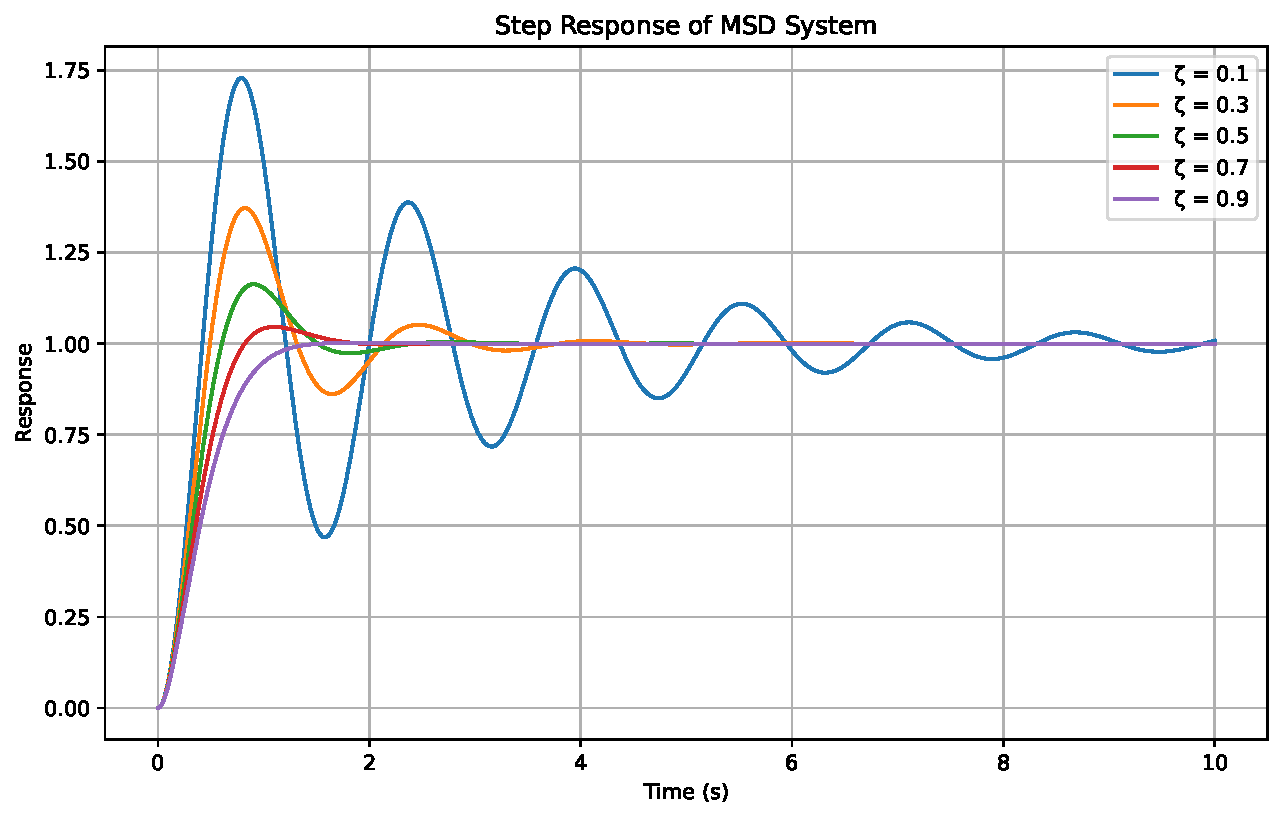
\includegraphics[keepaspectratio]{chapters/01_1-classical-control-highlights_files/figure-pdf/cell-3-output-1.pdf}}

In the case of the MSD system, we can find the poles of the transfer
function by finding the roots of the characteristic polynomial
\(D(s) = s^2 + 2\zeta\omega_n s + \omega_n^2\). The poles are given by:

\[ p_{1,2} = -\zeta\omega_n \pm j\omega_n\sqrt{1-\zeta^2} \]

or,

\[ p_{1,2} = -\zeta\omega_n \pm j\omega_d \]

where \(\omega_d = \omega_n\sqrt{1-\zeta^2}\) is the damped natural
frequency.

Finally, we can plot the poles of the MSD system for different values of
\(\zeta\).

\begin{Shaded}
\begin{Highlighting}[]
\ImportTok{import}\NormalTok{ numpy }\ImportTok{as}\NormalTok{ np}
\ImportTok{import}\NormalTok{ matplotlib.pyplot }\ImportTok{as}\NormalTok{ plt}

\NormalTok{zeta }\OperatorTok{=}\NormalTok{ [}\FloatTok{0.1}\NormalTok{, }\FloatTok{0.3}\NormalTok{, }\FloatTok{0.5}\NormalTok{, }\FloatTok{0.7}\NormalTok{, }\FloatTok{0.9}\NormalTok{]}
\NormalTok{wn }\OperatorTok{=} \DecValTok{4}

\CommentTok{\# Create a figure}
\NormalTok{plt.figure(figsize}\OperatorTok{=}\NormalTok{(}\DecValTok{10}\NormalTok{, }\DecValTok{6}\NormalTok{))}
\ControlFlowTok{for}\NormalTok{ z }\KeywordTok{in}\NormalTok{ zeta:}
    \CommentTok{\# Calculate poles}
\NormalTok{    p1 }\OperatorTok{=} \OperatorTok{{-}}\NormalTok{z}\OperatorTok{*}\NormalTok{wn }\OperatorTok{+} \OtherTok{1j}\OperatorTok{*}\NormalTok{wn}\OperatorTok{*}\NormalTok{np.sqrt(}\DecValTok{1}\OperatorTok{{-}}\NormalTok{z}\OperatorTok{**}\DecValTok{2}\NormalTok{)}
\NormalTok{    p2 }\OperatorTok{=} \OperatorTok{{-}}\NormalTok{z}\OperatorTok{*}\NormalTok{wn }\OperatorTok{{-}} \OtherTok{1j}\OperatorTok{*}\NormalTok{wn}\OperatorTok{*}\NormalTok{np.sqrt(}\DecValTok{1}\OperatorTok{{-}}\NormalTok{z}\OperatorTok{**}\DecValTok{2}\NormalTok{)}
\NormalTok{    plt.plot(np.real(p1), np.imag(p1), }\StringTok{\textquotesingle{}x\textquotesingle{}}\NormalTok{, label}\OperatorTok{=}\SpecialStringTok{f\textquotesingle{}ζ = }\SpecialCharTok{\{}\NormalTok{z}\SpecialCharTok{\}}\SpecialStringTok{\textquotesingle{}}\NormalTok{)}
\NormalTok{    plt.plot(np.real(p2), np.imag(p2), }\StringTok{\textquotesingle{}x\textquotesingle{}}\NormalTok{, label}\OperatorTok{=}\SpecialStringTok{f\textquotesingle{}ζ = }\SpecialCharTok{\{}\NormalTok{z}\SpecialCharTok{\}}\SpecialStringTok{\textquotesingle{}}\NormalTok{)}
\NormalTok{plt.xlabel(}\StringTok{\textquotesingle{}Real\textquotesingle{}}\NormalTok{)}
\NormalTok{plt.ylabel(}\StringTok{\textquotesingle{}Imaginary\textquotesingle{}}\NormalTok{)}
\NormalTok{plt.title(}\StringTok{\textquotesingle{}Poles of MSD System\textquotesingle{}}\NormalTok{)}
\NormalTok{plt.legend()}
\NormalTok{plt.grid(}\VariableTok{True}\NormalTok{)}
\NormalTok{plt.show()}
\end{Highlighting}
\end{Shaded}

\pandocbounded{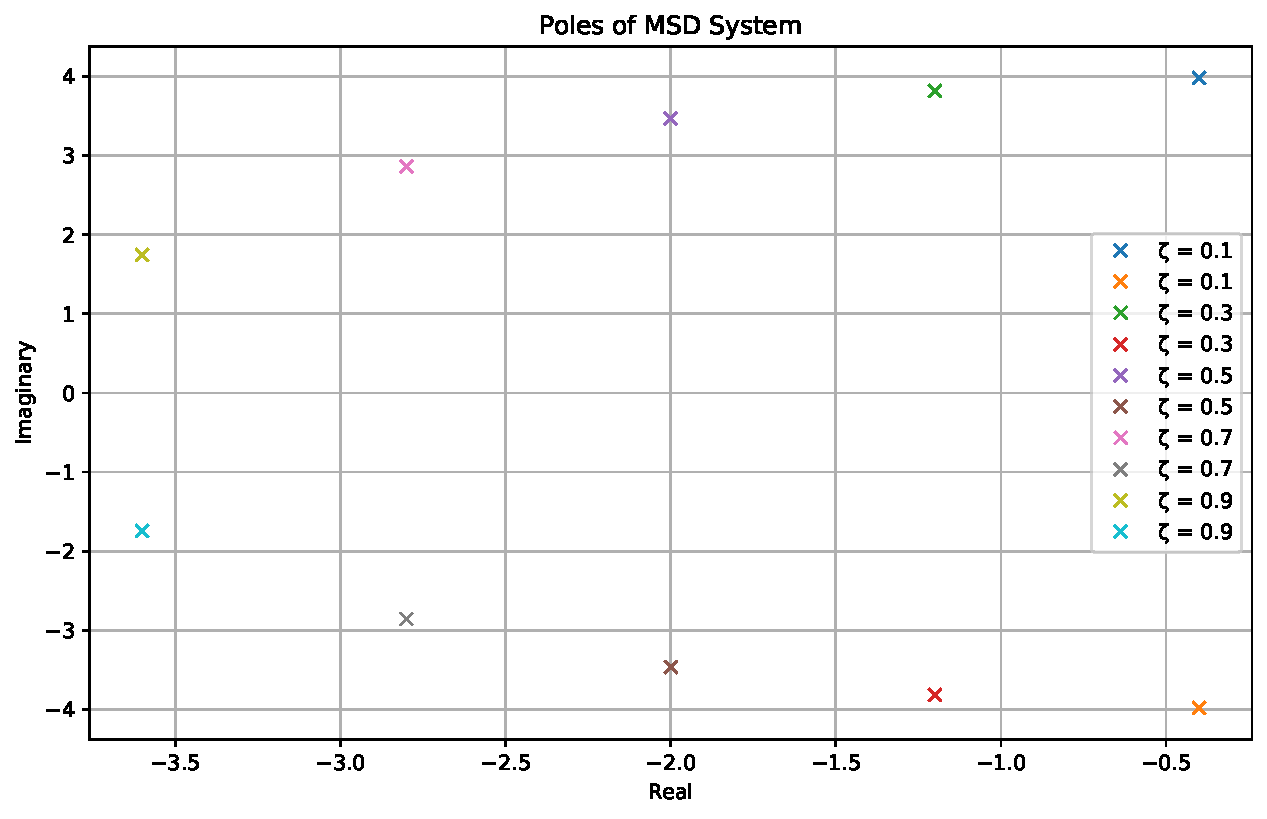
\includegraphics[keepaspectratio]{chapters/01_1-classical-control-highlights_files/figure-pdf/cell-4-output-1.pdf}}

If we plot the transfer function as a function of a single parameter, we
can see how the poles move in the complex plane as we change the damping
ratio \(\zeta\). This is known as a \emph{root locus} plot. We can plot
the root locus for any single variable.

What happens if the damping ratio is greater than 1? Or negative?

\section{Slide 11 - Performance of the MSD Step
Response}\label{slide-11---performance-of-the-msd-step-response}

Plot the step response and call out the different performance metrics,
such as rise time, settling time, overshoot, and steady-state error.
Discuss how these metrics are affected by the damping ratio \(\zeta\)
and natural frequency \(\omega_n\).

Add a figure showing the step response with annotations for rise time,
settling time, overshoot, and steady-state error.

\section{Slide 12 - Performance
Metrics}\label{slide-12---performance-metrics}

Performance:

{\def\LTcaptype{none} % do not increment counter
\begin{longtable}[]{@{}ll@{}}
\toprule\noalign{}
Quantity & Formula \\
\midrule\noalign{}
\endhead
\bottomrule\noalign{}
\endlastfoot
Rise Time & \(t_r=\frac{\pi-\beta}{\omega_d}\) \\
Peak Time & \(t_p=\frac{\pi}{\omega_d}\) \\
Overshoot & \(M_p=e^{-\pi\zeta/\sqrt{1-\zeta^2}}\) \\
Settling Time & \(t_s\approx\frac{4}{\zeta\omega_n}\) \\
\end{longtable}
}

Key point: \(\zeta\) and \(\omega_n\) tell us about performance and
stability of the sytem.

If we can use feedback to effectively change the poles of the system, we
can improve performance and stability.

\section{Slide 13 - Performance and Stability with
Feedback}\label{slide-13---performance-and-stability-with-feedback}

\subsection{Proportional Control}\label{proportional-control}

Draw a block diagram of a feedback control system with a plant \(G(s)\)
and a controller \(C(s)\). With \(C(s) = k_p\). Show how the closed-loop
transfer function is given by:

\[Y(s) = G(s)U(s)\]

Point out the idea of \emph{convolution} and the inverse Lapalce
Transform.

\[U(s) = C(s)E(s)\]

\[E(s) = U_r(s) - Y(s)\]

Therefore, we can write the closed-loop transfer function as:

\[Y(s) = G(s)C(s)E(s) = G(s)C(s)(U_r(s) - Y(s))\]

Solving for \(Y(s)\), we get:

\[Y(s) = \frac{G(s)C(s)}{1 + G(s)C(s)}U_r(s)\]

Draw \emph{closed loop} block diagram from \(U_r(s)\) to \(Y(s)\).

Now substitute \(C(s) = k_p\) and
\(G(s) = \frac{\omega_n^2}{s^2 + 2\zeta\omega_n s + \omega_n^2}\) to
get:

\[Y(s) = \frac{k_p\omega_n^2}{s^2 + 2\zeta\omega_n s + (1+k_p)\omega_n^2}U_r(s)\]

Notice the poles and Eigenvalues of the closed-loop system are a
function of the proportional gain \(k_p\). Therefore, we can use
feedback to change the poles of the system and improve performance and
stability.

\section{Slide 14 - Proportional
Feedback}\label{slide-14---proportional-feedback}

Let \(\overline{\omega}_n^2 = (1+k_p)\omega_n^2\) and
\(\overline{\zeta} = \frac{\zeta}{\sqrt{1+k_p}}\). Then we can write the
closed-loop transfer function as:

\[G_c(s) = \frac{k_p\omega_n^2}{s^2 + 2\overline{\zeta}\overline{\omega}_n s + \overline{\omega}_n^2}\]

\section{Slide 15 - Final Value
Theorem}\label{slide-15---final-value-theorem}

FVT: \(\lim_{t\to\infty} y(t) = \lim_{s\to0} sY(s)\)

Since the Laplace transform of the unit step function is \(U(s) = 1/s\),
we can use the final value theorem to write:

\[ \lim_{t\to\infty} y(t) = \lim_{s\to0} sY(s) = \lim_{s\to0} sG_c(s)U(s) = \lim_{s\to0} G_c(s) \]

\[ \lim_{t\to\infty} y(t) = \lim_{s\to0} G_c(s) = \lim_{s\to0} \frac{k_p\omega_n^2}{s^2 + 2\overline{\zeta}\overline{\omega}_n s + \overline{\omega}_n^2} = \frac{k_p}{\overline{\omega}_n^2}\]

\[ \lim_{t\to\infty} y(t) = \frac{k_p}{(1+k_p)} \ne 1\]

\section{Slide 16 - Proportional + Derivative
Feedback}\label{slide-16---proportional-derivative-feedback}

Now, since we have the closed loop Transfer Function, let's update the
control law to a \emph{PD} control law, where \(C(s) = k_p + k_d s\).

Notice with this control law, \(C(s)E(s) = k_p E(s) + k_d s E(s)\) and
in the time domain, this is equivalent to
\(u(t) = k_p e(t) + k_d \dot{e}(t)\).

Then we can write the closed-loop transfer function as:

\[G_c(s) = \frac{(k_p + k_d s)\omega_n^2}{s^2 + (2\zeta\omega_n + k_d\omega_n^2)s + (1+k_p)\omega_n^2}\]

Let \(\overline{\omega}_n^2 = (1+k_p)\omega_n^2\) and
\(\overline{\zeta} = \frac{2\zeta\omega_n + k_d\omega_n^2}{2\overline{\omega}_n}\),
then we can write the closed-loop transfer function as:

\[G_c(s) = \frac{(k_p + k_d s)\omega_n^2}{s^2 + 2\overline{\zeta}\overline{\omega}_n s + \overline{\omega}_n^2}\]

So we can modify the closed-loop damping ratio and natural frequency by
changing the proportional and derivative gains, \(k_p\) and \(k_d\). We
are also moving the poles around.

Notice we also added a zero which changes the transient response of the
system. The zero is located at \(s = -k_p/k_d\).

Finally, applying the final value theorem, we can see that the
steady-state error is still non-zero:

\[ \lim_{t\to\infty} y(t) = \lim_{s\to0} G_c(s) = \frac{k_p}{(1+k_p)} \]

\section{Slide 17 - Full PID
Feedback}\label{slide-17---full-pid-feedback}

Let \(C(s) = k_p + k_d s + \frac{k_i}{s}\), then we can write the
closed-loop transfer function as:

\[G_c(s) = \frac{(k_p + k_d s + \frac{k_i}{s})\omega_n^2}{s^2 + (2\zeta\omega_n + k_d\omega_n^2)s + (1+k_p)\omega_n^2 + k_i\omega_n^2}\]

or

\[G_c(s) = \frac{(k_d s^2 + k_p s + k_i)\omega_n^2}{s^3 + (2\zeta\omega_n + k_d\omega_n^2)s^2 + (1+k_p)\omega_n^2 s + k_i\omega_n^2}\]

Notice we added two zeros and a pole. Where are the new poles and zeros
located? How does this change the transient response of the system?

Plot the pzmap of the new closed-loop transfer function and discuss how
the poles and zeros have changed.

But applying the Final Value Theorem, we can see that the steady-state
error is now zero:

\[ \lim_{t\to\infty} y(t) = \lim_{s\to0} G_c(s) = 1 \]

There are many ways to tune a PID controller, but one of the most common
methods is the Ziegler-Nichols method. This method involves finding the
ultimate gain and ultimate period of the system, and then using these
values to calculate the PID gains.

We can also use the root locus method to tune a PID controller. This
method involves plotting the root locus of the system and then selecting
the desired closed-loop poles based on the desired performance
specifications.

Or we can use frequency response methods, such as Bode plots or Nyquist
plots, to tune a PID controller. These methods involve analyzing the
frequency response of the system and then selecting the PID gains based
on the desired performance specifications.

Or we can use optimization methods, such as genetic algorithms or
particle swarm optimization, to tune a PID controller. These methods
involve defining a cost function based on the desired performance
specifications and then using an optimization algorithm to find the PID
gains that minimize the cost function.

\bookmarksetup{startatroot}

\chapter{System Modeling}\label{system-modeling}

\section{Slide 2 - Motivation and Learning
Outcomes}\label{slide-2---motivation-and-learning-outcomes-2}

\subsection{\texorpdfstring{Developing a models is step
\emph{ZERO}}{Developing a models is step ZERO}}\label{developing-a-models-is-step-zero}

\begin{itemize}
\tightlist
\item
  Over the years several modeling techniques have been developed.
\item
  We want to explore their roots
\item
  Different methods have better (or worse) applications
\item
  In the Aero/Mechanical world we are generally concerned with:

  \begin{itemize}
  \tightlist
  \item
    Dynamics/Mechanics
  \item
    Vibrations
  \item
    ??
  \end{itemize}
\end{itemize}

\section{Slide 3 - The Heritage of
Mechanics}\label{slide-3---the-heritage-of-mechanics}

Free body diagrams and Newton's description of motion. The Principia:
mathematical principles of natural philosophy

\[\vec{F} = m \vec{a} = \frac{d}{dt} (m \vec{v})\]

For the MSD system,

\[m \ddot{q} + c \dot{q} + k q = f(t)\]

\section{Slide 4 - State, Time, and
Space}\label{slide-4---state-time-and-space}

We plot the response of the MSD system explicitly in time.

We can also plot the response in state space, where we plot the position
and velocity of the system as a function of time. This allows us to
visualize the dynamics of the system in a different way.

We can represent a system of higher order differential equations as a
system of first order differential equations. This is the basis of the
state space representation of a system.

This approach lends itself to numerical solving methods like
Runge-+Kutta and the tools of vector spaces and Real/Comples analysis.

\begin{tcolorbox}[enhanced jigsaw, arc=.35mm, bottomrule=.15mm, bottomtitle=1mm, breakable, colback=white, colbacktitle=quarto-callout-note-color!10!white, colframe=quarto-callout-note-color-frame, coltitle=black, left=2mm, leftrule=.75mm, opacityback=0, opacitybacktitle=0.6, rightrule=.15mm, title=\textcolor{quarto-callout-note-color}{\faInfo}\hspace{0.5em}{Note}, titlerule=0mm, toprule=.15mm, toptitle=1mm]

Do IC plot and Phase Plane Matlab example for the MSD system.

\end{tcolorbox}

\begin{itemize}
\tightlist
\item
  State Space gives a sense of flow and the vector field of the system
  for any initial conditions.
\item
  State Space gives a sense of the stability of the system, and how it
  will respond to perturbations.
\end{itemize}

\section{Slide 5 - The Heritage of Electrical
Engineering}\label{slide-5---the-heritage-of-electrical-engineering}

Fundational to this approach is the idea of input and output of a
system. Systems can be reduced to subsystems, etc., and analyzed as a
whole. This is the basis of the block diagram approach to modeling
systems.

\section{Slide 6 - Step and Frequency
Response}\label{slide-6---step-and-frequency-response}

We've talked about the step response from a performance perspective, but
we can also look at the step response from a modeling perspective. The
step response is a fundamental tool for understanding the dynamics of a
system.

The frequency response is another fundamental tool for understanding the
dynamics of a system. The frequency response tells us how the system
responds to different frequencies of input, and can be used to analyze
the stability and performance of the system.

Mostly we want to understand how the magnitude and phase of the output
changes with frequency. This is the basis of Bode plots, which are a
fundamental tool for analyzing the frequency response of a system.

\begin{tcolorbox}[enhanced jigsaw, arc=.35mm, bottomrule=.15mm, bottomtitle=1mm, breakable, colback=white, colbacktitle=quarto-callout-note-color!10!white, colframe=quarto-callout-note-color-frame, coltitle=black, left=2mm, leftrule=.75mm, opacityback=0, opacitybacktitle=0.6, rightrule=.15mm, title=\textcolor{quarto-callout-note-color}{\faInfo}\hspace{0.5em}{Note}, titlerule=0mm, toprule=.15mm, toptitle=1mm]

Do step response and Bode plot Matlab example for the MSD system.

\end{tcolorbox}

\section{Slide 7 - The Control View - State
Space}\label{slide-7---the-control-view---state-space}

\[ \frac{dx}{dt} = f(x, u), \ y = h(x, u) \]

\(x\) is the \emph{state} vector \(u\) is the \emph{input} vector \(y\)
is the \emph{output} vector

\(f\) is the \emph{state function} \(h\) is the \emph{output function}

These functions describe how the state of the system evolves over time,
and how the output of the system is related to the state and input.

With these functions and these views, it is natural to ask questions
like:

\begin{itemize}
\item
  Does the state converge? (Stability)
\item
  What states can the system reach given the proper choice of u(t)?
  (controllability or reachability)
\item
  If we don't measure the whole state, can we reconstruct the state?
  (observability)
\item
  Notice the answers to these questions should not depend on the system
  we are working with, but on properties of the model
\end{itemize}

\section{Slide 8 - Summary}\label{slide-8---summary}

\bookmarksetup{startatroot}

\chapter{State Space Modeling}\label{state-space-modeling}

\section{Slide 2 - Motivation and Learning
Outcomes}\label{slide-2---motivation-and-learning-outcomes-3}

\subsection{The Fundamental
Abstraction}\label{the-fundamental-abstraction}

\begin{itemize}
\tightlist
\item
  Dynamic System Theory as a branch of mathematics gives us a
  foundational starting point
\item
  We will rely on a variety of math tools, but primarily Linear Algebra
  and Analysis
\end{itemize}

\section{Slide 3 - Start with ODEs}\label{slide-3---start-with-odes}

Let:

\[\dot{\underline{x}} = \underline{f}(\underline{x},\underline{u},t) \\
y = \underline{h}(\underline{x},\underline{u},t)\]

Where \(\underline{x} \in \mathbb{R}^n\) is the state vector,
\(\underline{u} \in \mathbb{R}^q\) is the input vector, and
\(y \in \mathbb{R}^p\) is the output/measurement vector. The function
\(\underline{f}\) describes how the state evolves over time, while
\(\underline{h}\) describes how the output is generated from the state
and input.

and \(\underline{f}: \mathbb{R}^n \times \mathbb{R}^p \to \mathbb{R}^n\)
and \(\underline{h}: \mathbb{R}^n \times \mathbb{R}^p \to \mathbb{R}^q\)
are vector-valued functions that describe the dynamics of the system.

\emph{This is the State Space Model of a system.}

\section{Slide 4 - For LTI systems}\label{slide-4---for-lti-systems}

We have the LTI State Space Model:

\[\dot{\underline{x}} = A \underline{x} + B \underline{u} \\
y = C \underline{x} + D \underline{u}\]

Where \(A \in \mathbb{R}^{n \times n}\) is the state or dynamics matrix,
\(B \in \mathbb{R}^{n \times q}\) is the input or control matrix,
\(C \in \mathbb{R}^{p \times n}\) is the output or measurement matrix,
and \(D \in \mathbb{R}^{p \times q}\) is the feedthrough or direct
matrix.

The matrices \(A\), \(B\), \(C\), and \(D\) are constant for LTI
systems.

\section{Slide 7 - Example - The Inverted
Pendulum}\label{slide-7---example---the-inverted-pendulum}

\begin{tcolorbox}[enhanced jigsaw, arc=.35mm, bottomrule=.15mm, bottomtitle=1mm, breakable, colback=white, colbacktitle=quarto-callout-note-color!10!white, colframe=quarto-callout-note-color-frame, coltitle=black, left=2mm, leftrule=.75mm, opacityback=0, opacitybacktitle=0.6, rightrule=.15mm, title=\textcolor{quarto-callout-note-color}{\faInfo}\hspace{0.5em}{Note}, titlerule=0mm, toprule=.15mm, toptitle=1mm]

Draw a figure of the inverted pendulum. Theta is defined positive
counter-clockwise from vertical.

\end{tcolorbox}

\[J_t\ddot{\theta} + \gamma\dot{\theta} - mgl\sin(\theta) = u\]

Where \(J_t = J + ml^2\) is the total moment of inertia of the pendulum
about the pivot point, \(\gamma\) is the damping coefficient, \(m\) is
the mass of the pendulum, \(g\) is the acceleration due to gravity,
\(l\) is the length of the pendulum, and \(u\) is the control input
(torque applied at the pivot point).

\section{Slide 8 - State Space Model of the Inverted
Pendulum}\label{slide-8---state-space-model-of-the-inverted-pendulum}

Let
\(\underline{x} = \begin{bmatrix} \theta \\ \dot{\theta} \end{bmatrix}\),
then we can write the state space model as:

\[ \dot{\underline{x}} = \begin{bmatrix} \dot{\theta} \\ \ddot{\theta} \end{bmatrix} = \begin{bmatrix} \dot{\theta} \\ -\frac{\gamma}{J_t}\dot{\theta} + \frac{mgl}{J_t}\sin(\theta) + \frac{u}{J_t} \end{bmatrix} \]

Where
\(\underline{f}(\underline{x},\underline{u}) = \begin{bmatrix} \dot{\theta} \\ -\frac{\gamma}{J_t}\dot{\theta} + \frac{mgl}{J_t}\sin(\theta) + \frac{u}{J_t} \end{bmatrix}\).

Now say we measure the horizontal displacement \(d\). That gives,

\[\underline{y} = l\sin(\theta)\]

Where \(\underline{h}(\underline{x},\underline{u}) = l\sin(\theta)\).

\section{Slide 9 - Linearization of the Inverted
Pendulum}\label{slide-9---linearization-of-the-inverted-pendulum}

When \(\theta \approx 0\), we can linearize the system about the
equilibrium point \(\theta = 0\) to obtain the LTI state space model:

\[\dot{\underline{x}} = \begin{bmatrix} 0 & 1 \\ \frac{mgl}{J_t} & -\frac{\gamma}{J_t} \end{bmatrix} \underline{x} + \begin{bmatrix} 0 \\ \frac{1}{J_t} \end{bmatrix} u\]

\[\underline{y} = \begin{bmatrix} l & 0 \end{bmatrix} \underline{x}\]

Where
\(A = \begin{bmatrix} 0 & 1 \\ \frac{mgl}{J_t} & -\frac{\gamma}{J_t} \end{bmatrix}\)
and \(B = \begin{bmatrix} 0 \\ \frac{1}{J_t} \end{bmatrix}\) and
\(C = \begin{bmatrix} l & 0 \end{bmatrix}\) and \(D = 0\).

\section{Slide 10 - Simulink Example of the Inverted
Pendulum}\label{slide-10---simulink-example-of-the-inverted-pendulum}

\section{Slide 11 - Block Diagrams
Overview}\label{slide-11---block-diagrams-overview}

\section{Slide 12 - Summary}\label{slide-12---summary}

\subsection{\texorpdfstring{Developing a model is step \emph{ZERO} in
the design of a control
system.}{Developing a model is step ZERO in the design of a control system.}}\label{developing-a-model-is-step-zero-in-the-design-of-a-control-system.}

\begin{itemize}
\tightlist
\item
  Modeling is a key step in developing a control system analysis

  \begin{itemize}
  \tightlist
  \item
    Without the model, we have no place to start
  \end{itemize}
\item
  The State Space approach is generally considered a good place to start
\item
  We will use a variety of modeling tools

  \begin{itemize}
  \tightlist
  \item
    Math, linear analysis, ODEs,
  \item
    Block diagrams
  \item
    Matlab and Simulink
  \item
    Python *\ldots{}
  \end{itemize}
\item
  ``All models are wrong, but some are useful.'' -- George E. P. Box
\end{itemize}

\bookmarksetup{startatroot}

\chapter{Time Response}\label{time-response}

\section{Learning Objectives}\label{learning-objectives}

\begin{itemize}
\tightlist
\item
  Analyze second-order systems
\item
  Compute rise time, overshoot, settling time
\end{itemize}

\bookmarksetup{startatroot}

\chapter{Feedback Control}\label{feedback-control}

\section{Learning Objectives}\label{learning-objectives-1}

\begin{itemize}
\tightlist
\item
  Derive closed-loop transfer functions
\end{itemize}

\bookmarksetup{startatroot}

\chapter{Root Locus}\label{root-locus}

\section{Learning Objectives}\label{learning-objectives-2}

\begin{itemize}
\tightlist
\item
  Sketch root loci
\end{itemize}

\bookmarksetup{startatroot}

\chapter{Frequency Response}\label{frequency-response}

\section{Learning Objectives}\label{learning-objectives-3}

\begin{itemize}
\tightlist
\item
  Bode plots
\item
  Nyquist criterion
\end{itemize}

\bookmarksetup{startatroot}

\chapter{PID Design}\label{pid-design}

\section{Learning Objectives}\label{learning-objectives-4}

\begin{itemize}
\tightlist
\item
  Tune P, PI, PD, PID controllers
\end{itemize}




\end{document}
